% Autor: Leonhard Segger, Alexander Neuwirth
% Datum: 2017-10-30
\documentclass[
	% Papierformat
	a4paper,
	% Schriftgröße (beliebige Größen mit „fontsize=Xpt“)
	12pt,
	% Schreibt die Papiergröße korrekt ins Ausgabedokument
	pagesize,
	% Sprache für z.B. Babel
	ngerman
]{scrartcl}

% Achtung: Die Reihenfolge der Pakete kann (leider) wichtig sein!
% Insbesondere sollten (so wie hier) babel, fontenc und inputenc (in dieser
% Reihenfolge) als Erstes und hyperref und cleveref (Reihenfolge auch hier
% beachten) als Letztes geladen werden!

% Silbentrennung etc.; Sprache wird durch Option bei \documentclass festgelegt
\usepackage{babel}
% Verwendung der Zeichentabelle T1 (Sonderzeichen etc.)
\usepackage[T1]{fontenc}
% Legt die Zeichenkodierung der Eingabedatei fest, z.B. UTF-8
\usepackage[utf8]{inputenc}
% Schriftart
\usepackage{lmodern}
% Zusätzliche Sonderzeichen
\usepackage{textcomp}

% Mathepaket (intlimits: Grenzen über/unter Integralzeichen)
\usepackage[intlimits]{amsmath}
% Ermöglicht die Nutzung von \SI{Zahl}{Einheit} u.a.
\usepackage{siunitx}
% Zum flexiblen Einbinden von Grafiken (\includegraphics)
\usepackage{graphicx}
% Abbildungen im Fließtext
\usepackage{wrapfig}
% Abbildungen nebeneinander (subfigure, subtable)
\usepackage{subcaption}
% Funktionen für Anführungszeichen
\usepackage{csquotes}
% Zitieren, Bibliographie
\usepackage{biblatex}


% Zur Darstellung von Webadressen
\usepackage{url}
%chemische Formeln
\usepackage[version=4]{mhchem}
% siunitx: Deutsche Ausgabe, Messfehler getrennt mit ± ausgeben
\usepackage{floatrow}
\floatsetup[table]{capposition=top}
% Verlinkt Textstellen im PDF-Dokument
\usepackage[unicode]{hyperref}
% "Schlaue" Referenzen (nach hyperref laden!)
\usepackage{cleveref}
\sisetup{
	locale=DE,
	separate-uncertainty
}
%\bibliography{6Mi_S2_25-10-2017_References}

\begin{document}
	
	\begin{titlepage}
		\centering
		{\scshape\LARGE Versuchsbericht zu \par}
		\vspace{1cm}
		{\scshape\huge M3 - Elaszizität\par}
		\vspace{2.5cm}
		{\LARGE Gruppe 6Mi \par}
		\vspace{0.5cm}
		
		{\large Alexander Neuwirth (E-Mail: a\_neuw01@wwu.de) \par}
		{\large Leonhard Segger (E-Mail: l\_segg03@uni-muenster.de) \par}
		\vfill
		
		durchgeführt am 29.11.2017\par
		betreut von\par
		{\large Christian Thiede}
		
		\vfill
		
		{\large \today\par}
	\end{titlepage}
	\tableofcontents
	\newpage
	
	\section{Kurzfassung}
	***Kurzfassung\\
	

	\section{Methoden}
	***Methoden \\
	*** Paralaxen frei wegen spiegel
	*** Schwing MEsspunkt bei max. Speed
	*** Gewichte als exakt angenommen
	
	
	\section{Ergebnisse und Diskussion}

	\subsection{Beobachtung}
	*** linear-> Fit und Algorithmus angeben \\
	*** Biegungen in einen Graphen \\
	*** Graphen beschreiben \\
	*** Unsicherheitenrechnung \\

	\subsection*{Daten}
	\begin{figure}[H]
		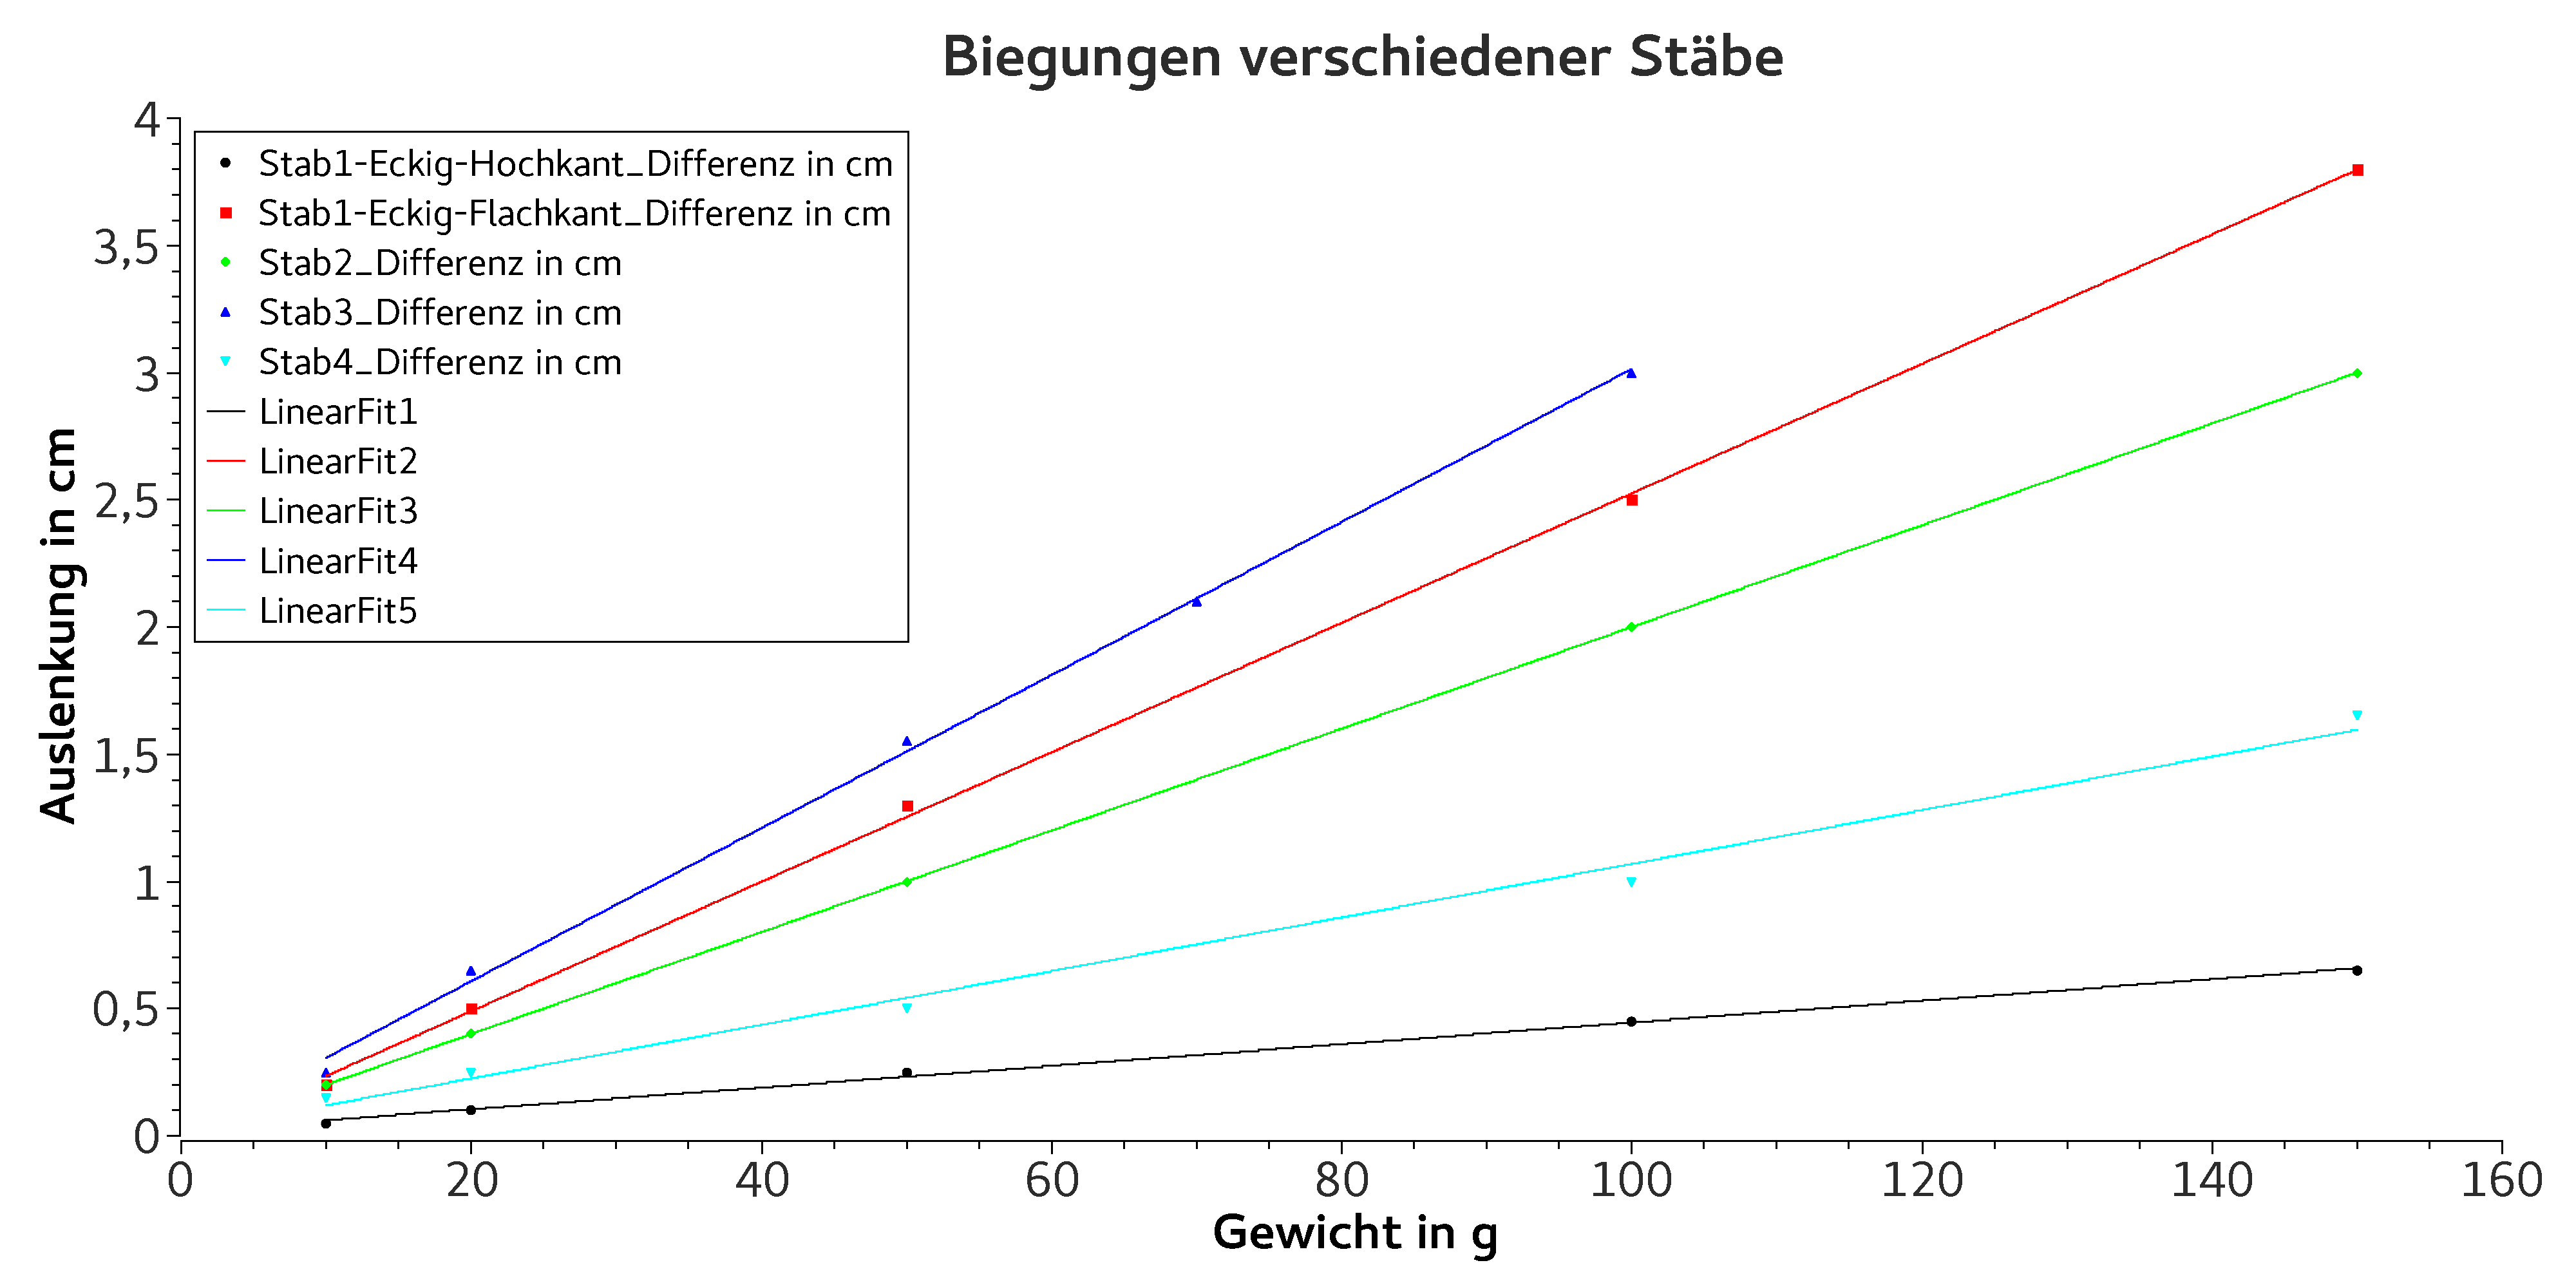
\includegraphics[width=1\textwidth]{Biegungen}
		\centering
		\caption{Biegungen verschiedener Stäbe}
		\label{BiegungGraph}
		\centering
	\end{figure}

	\begin{table}[H]
	\centering
	\begin{tabular}{ l | c | c | c | c | c |}
		& S1 hochkant  & S1 flachkant & S2 & S3 & S4  \\ \hline
		a in \SI{}{\centi\meter\per\gram} & $\SI{0,004264}{}$& $ \SI{0,025452}{}$&  $ \SI{0,02}{}$ & $\SI{0,030093}{}$ & $\SI{0,0105466}{}$  \\ \hline
		b in \SI{}{\centi\meter} & $\SI{0,018586}{}$  & $\SI{-0,019825}{}$  &  $\SI{-2e-17}{}$ &  $\SI{0,005370}{}$&  $\SI{0,013921}{}$   \\ \hline
	\end{tabular}
	\caption{Parameter die beim Fitten sich ergeben}
	\label{TabelleFits}
	\end{table}

	\subsection*{Unsicherheiten}
	\begin{table}[H]
	\centering
	\begin{tabular}{ l | c | c | c | c |}
		& Mikroschraube  & Massband/Biegungsanzeige & Stoppuhranzeige & Reaktionszeit \\ \hline
		u  & $\SI{0,00577}{cm}$ &  $\SI{0,05774}{cm}$ &  $\SI{0,005774}{s}$ &  $\SI{0,11547}{s}$  \\ \hline
	\end{tabular}
	\caption{Unsicherheiten der verwendeten Messinstrumente. Die Wahrscheinlichkeitsdichtefunktionen wurden als rechteckig angenommen.}
		\label{TabelleUnsicherheiten}
	\end{table}

	\subsection{Diskussion}

	
	\section{Schlussfolgerung}
	***Materialien vergleich mit Literatur \\
	
	
	%\printbibliography
\end{document}
